\chapter{State of the Art}
\label{chap:Chapter2}
In this chapter, it will be presented an overview of \glspl{uav}, the fundamentals of propellers, fixed-pitch propellers and variable-pitch propellers.

%-------------------------------------------------------------------------------%
\section{Unmanned Aerial Vehicle}
\glspl{uav}, commonly known as drones, have gathered significant attention in both civil and military operations due to their exceptional mobility, enhanced stability, cost-effectiveness, and endurance across various tasks.
They can be found in applications of diverse fields such as logistics, forest monitoring, construction, freight transportation, communication, healthcare, post-disaster operations, search and rescue, remote sensing, precision agriculture, power-line inspection, traffic surveillance, as well as object detection and tracking \cite{UAV1}, \cite{UAV5}, \cite{UAV14}.

In essence, \glspl{uav} are unmanned aerial vehicles, capable of autonomous and remote operation..
They rely on communication links to connect with ground control stations.
Remote operation typically involves a human operator monitoring and/or controlling the \gls{uav} through a remote control \cite{UAV5}, \cite{UAV14}.

Given the widespread interest in drones, numerous \glspl{uav} of varying sizes and forms (illustrated in Figure \ref{fig:UAV_examples}) have been developed to fulfill a range of tasks \cite{UAV5}, \cite{UAV13}, \cite{UAV14}.

Each type of \gls{uav} comes with its own set of advantages and disadvantages, guiding the selection based on the specific application requirements \cite{UAV5}, \cite{UAV13}, \cite{UAV14}.

\begin{figure}[H]
    \centering
    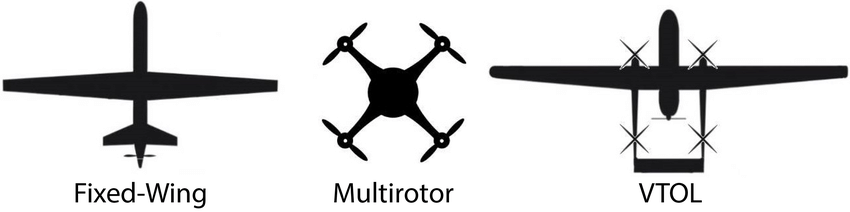
\includegraphics[scale=0.45]{ch2/assets/UAV_examples.png}
    \caption{Examples of UAV types \cite{UAV13}}
    \label{fig:UAV_examples}
\end{figure}


\subsection{Propeller Fundamentals}
The purpose of a propeller is to convert the rotational power produced by the engine into forward thrust during flight.
This is achieved by accelerating a mass of air through the blades of the propeller as it spins, generating the necessary force to propel the aircraft forward at a specific airspeed \cite{main_uav}.
Figure \ref{fig:propeller}, illustrates the connection between the changing the propeller rotation speed and the speed and movement.

\begin{figure}[H]
    \centering
    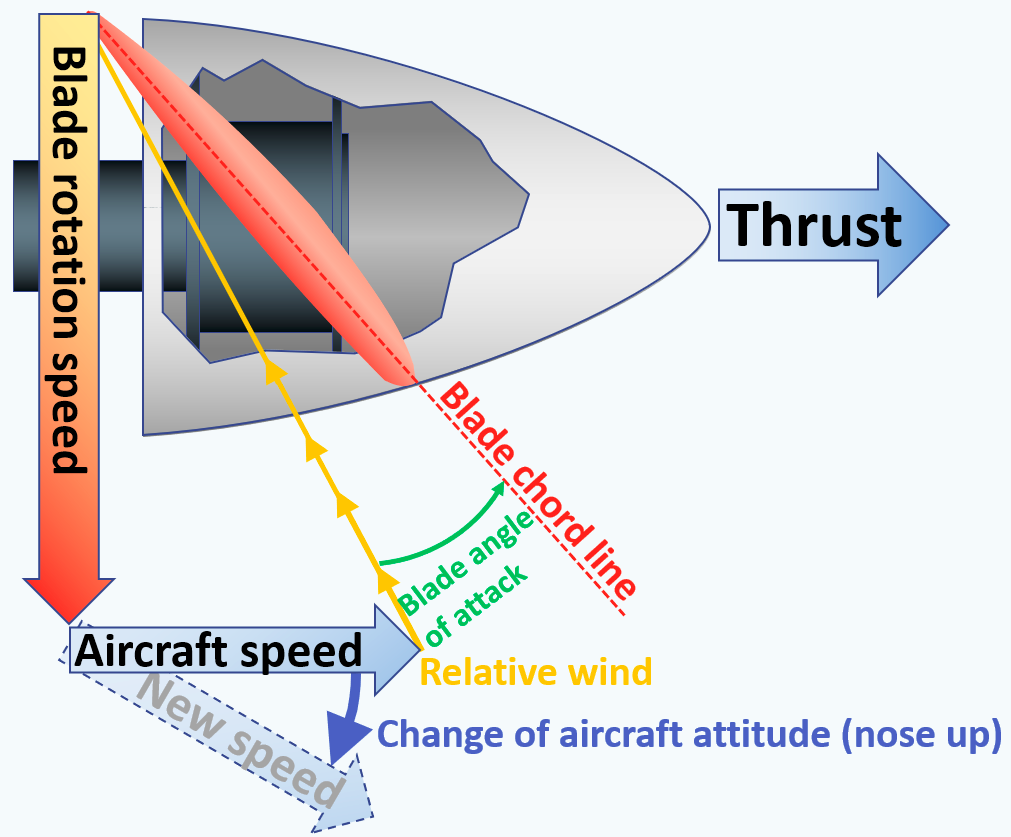
\includegraphics[scale=0.25]{ch2/assets/propeller.png}
    \caption{Propeller blade representation \cite{propeller}}
    \label{fig:propeller}
\end{figure}

The propeller performance can be affected by \cite{main_uav}:
\begin{itemize}
    \item Blade diameter
    \item Number of blades
    \item Blade pitch
\end{itemize}

While the propeller diameter affects lift efficiency (higher diameter, higher efficiency), the number of blades affects the thrust \cite{main_uav}.

As for the propeller pitch, it is considered as the distance that a propeller moves forward in one revolution.
A higher pitch allows the propeller to move the aircraft faster through the air and while a lower pitch results in less forward movement but may be more suitable for applications where lower speeds or higher thrust are required \cite{main_uav}.

This means that each flight phase requires a different propeller pitch\cite{main_uav}:
\begin{itemize}
    \item Take-off - Fine Pitch
    \item Hover - Finest Pitch
    \item Flight - Coarse pitch
    \item Landing - Fine Pitch
\end{itemize}

\subsection{Fixed Pitch Proprotors}
Fixed-pitch propellers, as the name suggests, have a predetermined blade pitch that remains constant during operation.
The design, like the example in figure \ref{fig:prop_2}, involves selecting an ideal blade pitch based on the combination of motor angular speed and airspeed at which the propeller operates.

\begin{figure}[H]
    \centering
    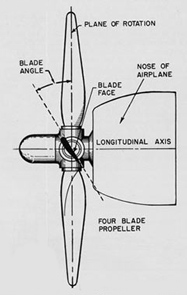
\includegraphics[scale=0.8]{ch2/assets/prop_2.jpg}
    \caption{Example of Fixed Pitch \cite{FPP8}}
    \label{fig:prop_2}
\end{figure}

To address varying thrust requirements at different airspeeds, it is possible to choose between a fine fixed-pitch propeller for take-off and climb and a coarse one for cruise.

While simple to operate, fixed-pitch propellers require alignment of factors such as motor \gls{RPM}, airspeed, relative airflow, blade pitch, diameter, number of blades, blade chord and length.
This design proves inefficient for various flight modes \cite{main_uav}, \cite{FPP6}, \cite{FPP7}.

\subsection{Variable Pitch Proprotors}
Historically, early aviation pioneers experimented with propellers that could only be adjusted on the ground.
The Gloster Hele-Shaw Beacham Variable Pitch Propeller (VPP), developed in 1928, demonstrated practical controllable pitch capabilities.
Over time, various designs and mechanisms, including hydraulic and pneumatic systems, were explored and refined.
The development of constant-speed propellers marked a significant advancement in aviation technology, offering improved efficiency and performance \cite{VPP2}.

A significant advantage of VPP is its ability to adapt to varying airspeeds.
When an aircraft is stationary or moving slowly, the propeller blades can be set to a low angle of attack to reduce drag.
As the aircraft gains speed, the pitch is increased to maintain optimal performance.
This adaptability ensures efficient operation across a range of flight conditions \cite{main_uav}, \cite{VPP1}.

The primary purpose of VPPs is to maintain the optimal angle of attack relative to the changing wind vector as the aircraft accelerates.
Traditional fixed-pitch propellers face efficiency challenges in various flight conditions.
Adjustable blade angles address this issue, allowing for improved efficiency during takeoff and cruise \cite{VPP2}, \cite{VPP3}.

Variable-pitch systems, like in figure \ref{fig:vpp_example}, can adjust blade pitch to maintain a selected \gls{RPM} enhancing overall performance, especially at high altitudes, by allowing the rotor to operate in its most economical speed range \cite{VPP2}, \cite{VPP3}.

\begin{figure}[H]
    \centering
    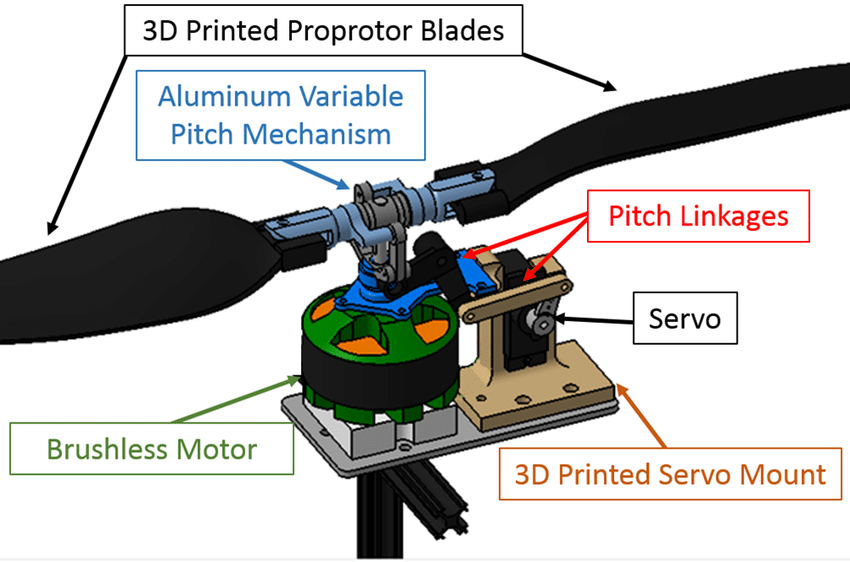
\includegraphics[scale=0.4]{ch2/assets/vpp_example.png}
    \caption{Example of Variable Pitch Mechanism \cite{VPP4}}
    \label{fig:vpp_example}
\end{figure}

There are three methods to change the pitch: Hydraulic, Centrifugal, and Electromechanical control \cite{VPP2}.

\subsubsection{Hydraulic Method}
This system involves the use of engine oil pressure to control the pitch-changing mechanism, as it is possible to see in figures \ref{fig:vpp_hydro1} and \ref{fig:vpp_hydro2}.
It consists of a pump, control valves, and cylinders that actuate the movement of the propeller blades \cite{VPP2}, \cite{VPP8}..

Hydraulic systems provide a precise means of adjusting the propeller pitch, allowing efficient performance under different flight conditions, and contributing to the overall safety and reliability of the system \cite{VPP5}.

But Hydraulic systems add complexity and weight to the overall aircraft system.
More components means more elements could potentially fail or require maintenance.
Hydraulic systems also have a slow response time due to the time it takes for hydraulic pressure changes to propagate through the system \cite{VPP2}, \cite{VPP8}..

\begin{figure}[H]
    \centering
    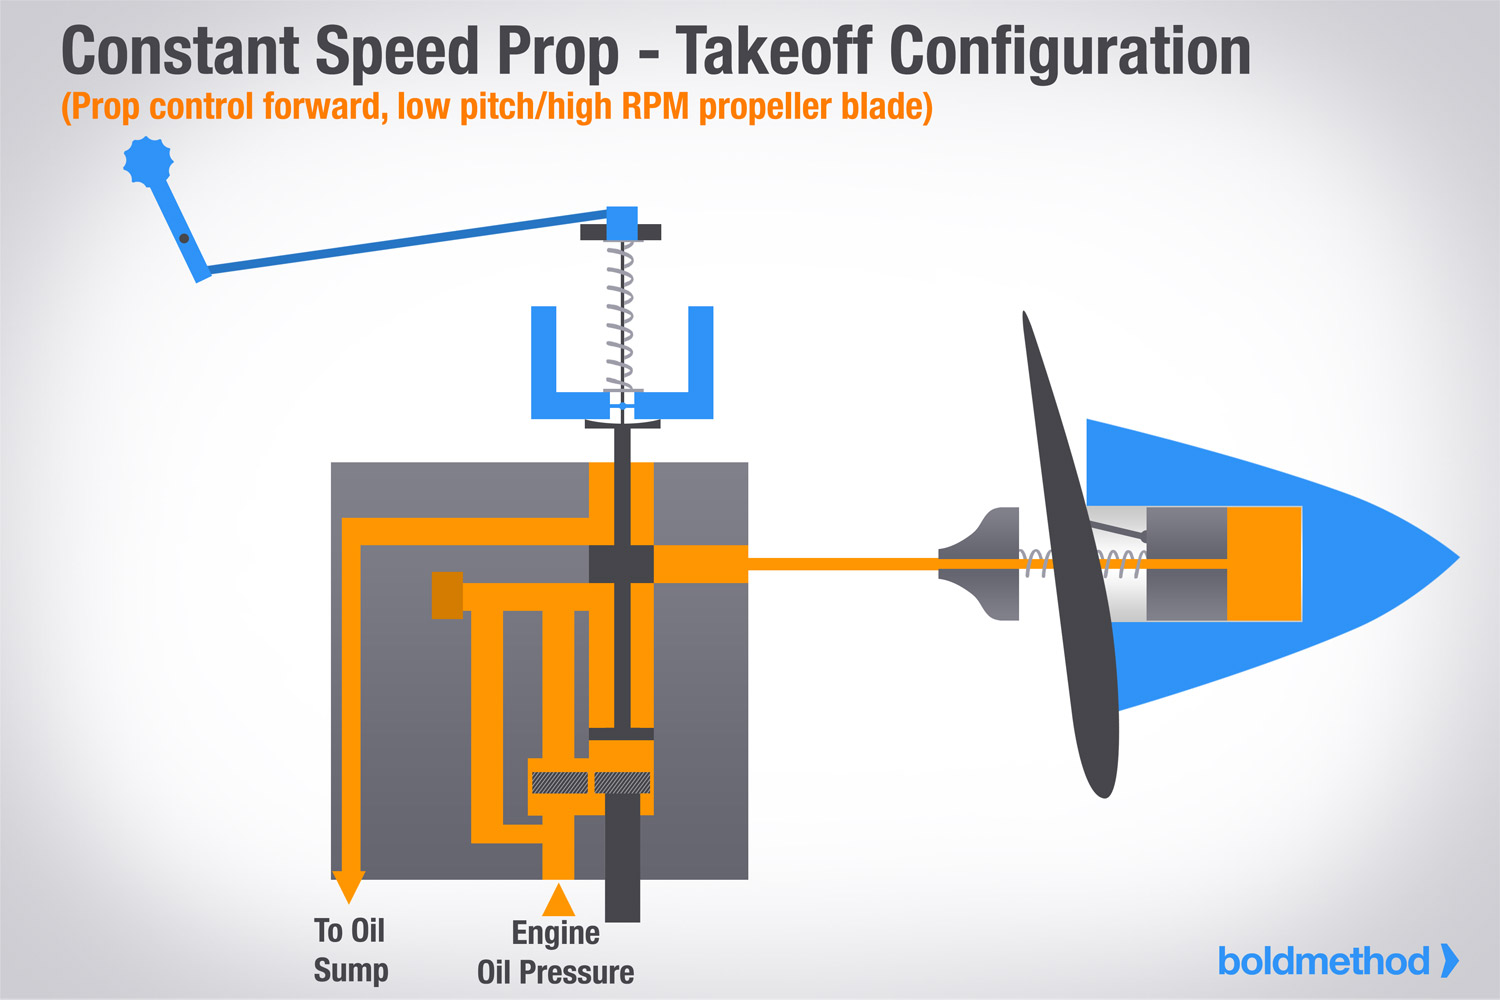
\includegraphics[scale=0.25]{ch2/assets/vpp_hydro1.jpg}
    \caption{VPP Hydraulic Method - Takeoff \cite{VPP5}}
    \label{fig:vpp_hydro1}
\end{figure}

\begin{figure}[H]
    \centering
    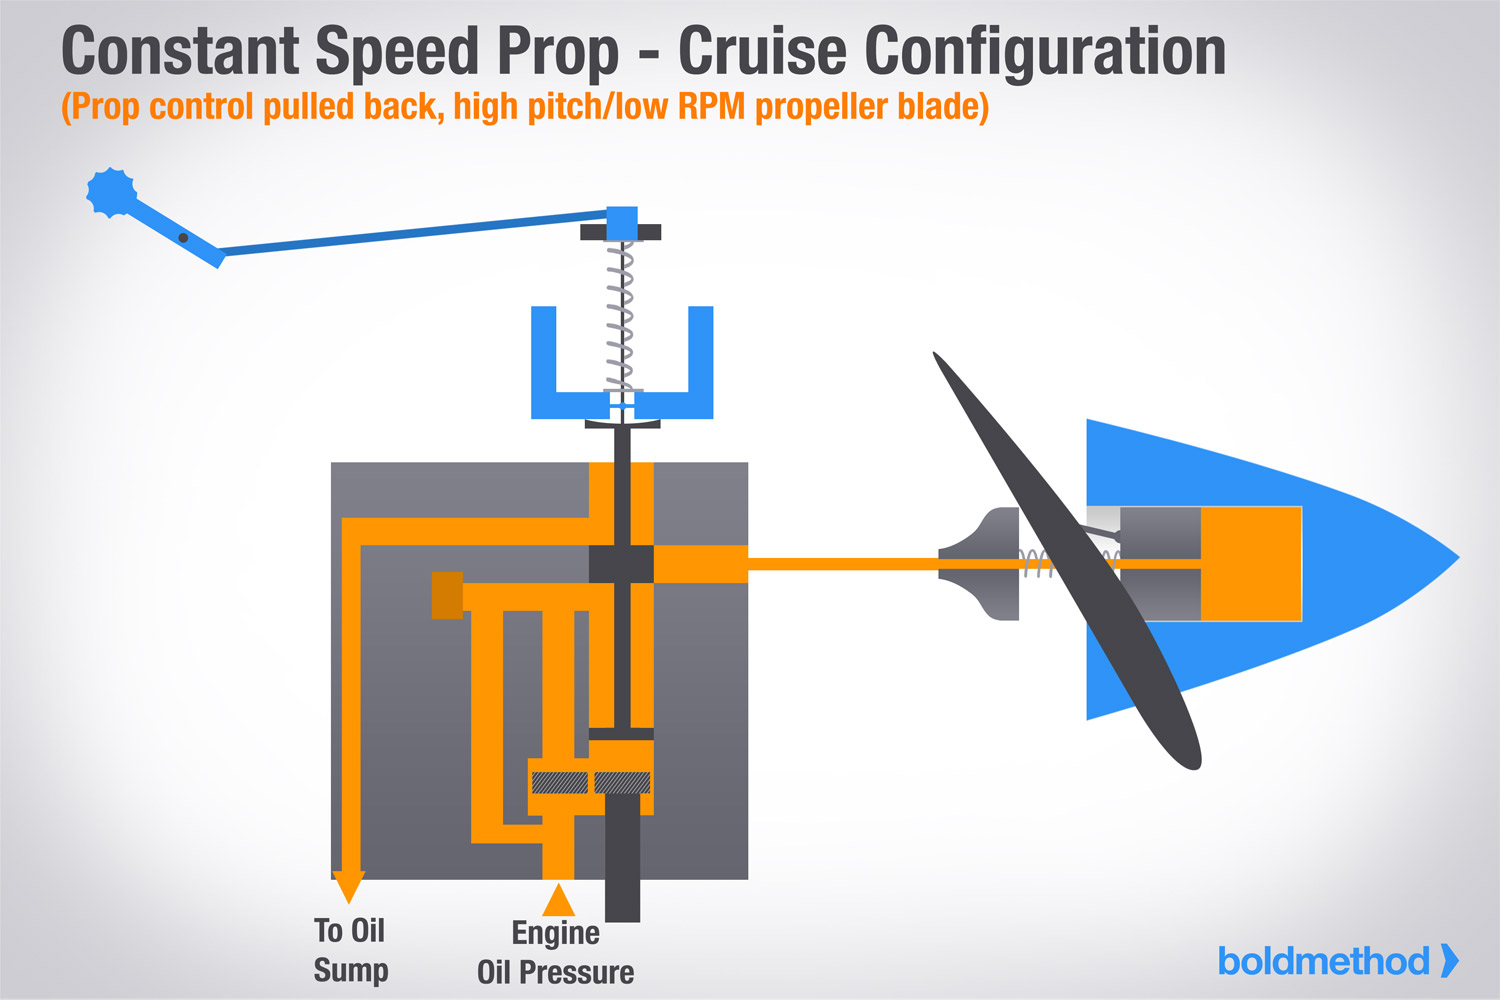
\includegraphics[scale=0.25]{ch2/assets/vpp_hydro2.jpg}
    \caption{VPP Hydraulic Method - Cruise \cite{VPP5}}
    \label{fig:vpp_hydro2}
\end{figure}

\subsubsection{Centrifugal Method}
In the centrifugal systems, centrifugal weights are attached directly to the propellers.
An eccentric weight is placed near or in the spinner and secured with a spring and, when the propeller reaches a certain \gls{RPM}, centrifugal force swings the weights outward, driving a mechanism that twists the propeller to a steeper pitch.
As the propeller slows down, the \gls{RPM} drops and the spring pushes the weight back, readjusting the propeller pitch to a shallower pitch.

As advantages, centrifugal systems are simpler compared to hydraulic systems since they involve fewer components.
There is no need to use external power sources, such as an engine-driven pump.
Also, centrifugal systems can operate automatically without direct pilot intervention.

As disadvantages, centrifugal systems may provide less precise pitch control than more advanced hydraulic or electronic systems.
The response time of centrifugal systems may be slower compared to more sophisticated systems \cite{VPP2}.

\subsubsection{Electromechanical Method}
These systems involve electric motors and mechanical linkages to control the pitch of the propeller blades \cite{VPP8}.
Figures \ref{fig:vpp_example} and \ref{fig:vpp_electric} and this \href{https://www.youtube.com/watch?v=MpsBOQOUB-4}{\textit{VPP Electromechanical Method Video}} illustrates the components and functionality of this method.

\begin{figure}[H]
    \centering
    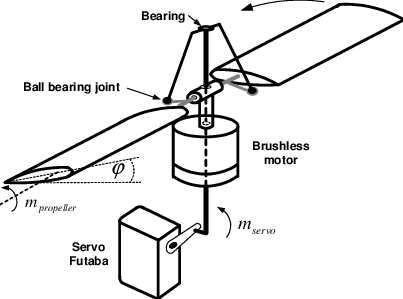
\includegraphics[scale=0.6]{ch2/assets/vpp_electric.png}
    \caption{VPP Electromechanical Method \cite{VPP6}}
    \label{fig:vpp_electric}
\end{figure}

Electromechanical methods provide precise control over the pitch of the propeller blades, can offer rapid response times to changes in flight conditions, are often versatile, and can be adapted for various aircraft configurations.
They often have fewer components prone to wear and can be more straightforward \cite{VPP8}.

However electromechanical systems, including motors and associated components, can add weight to the aircraft, require electrical power to operate, and are more complex than purely mechanical systems, increasing the chance of failures \cite{VPP2}, \cite{VPP8}.

%-------------------------------------------------------------------------------%
